%!TEX root = ../main.tex
\section{Introduction}
For this master thesis, we want to be able to analyse the difference between several data structures. Moreover, the traditional adjacency matrix is not adapted for the big graphs. Indeed the neighbourhood of a vertex is obtain in $O(|V|)$ given that it is necessary to go through the entire line. Furthermore, when the graph is not dense, a big part of the used memory is useless.

As a reminder, an adjacency matrix is a two dimension array, where each line represents a starting vertex and each column represents a ending vertex. The values represent the capacity between both vertices, 0 meaning that there are no edge between them. \newline

\begin{figure}[!h]
\begin{subfigure}{.6\textwidth}
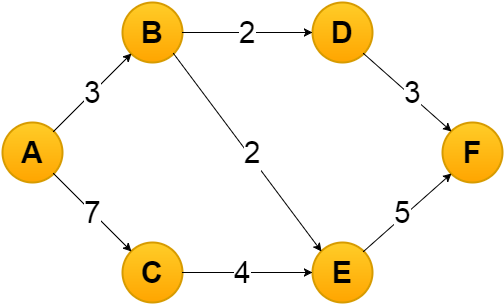
\includegraphics[width=7.5cm,height=4.5cm]{images/graph.png}
\end{subfigure}
\begin{subfigure}{.4\textwidth}
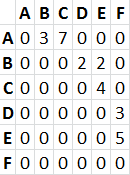
\includegraphics[scale=0.7]{images/adjacencyMatrix.png}
\end{subfigure}
\caption{A graph with its adjacency matrix.}
\end{figure}

We thus decide to use an other structure; \newline

With the same principle as the adjacency matrix, we use an array where each line represents the neighbours of a vertex. For example, the first line contains the information on the neighbours of the first vertex. But contrary to the adjacency matrix, we do not use an array to represent neighbours but a different structure requiring less memory space. \newline

We used five different data structures : hash map, tree map, simple linked list and two home-made structures based on the sparse set, split array and sparse map. 

Each vertex will have its structure, storing which vertices are neighbours and what are the capacities of the edges to these vertices. If we had to represent a graph with 10 vertices, we would have a array of 10, for example, hash map. Each hash map representing the neighbourhood of a single vertex.

\section{Data structures}
\subsection{Hash Map}
A hash map is an unordered associative array, which associates a key with a value. It contains a single array of buckets, where the values are stored. A hash function converts the key into an index, which represents the bucket where the record (key/value) is stored. \newline

Ideally, the hash function assigns to every key a different bucket but it is possible to have several keys giving the same hash code. This is called a \textit{collision}. One bucket can thus contain several records. \newline

The \textit{load factor} is the number of records divided by the number of buckets.  If the load factor is too high, the hash map will be slower. But having a too low load factor does not save search time, it just uses some memory pointlessly. To keep the load factor to a defined value (eg between $\frac{2}{3}$ and $\frac{3}{4}$), we must, when inserting new records, resize the hash map. \newline

In our case, the key is the id of the nearby vertex and the value is the capacity of the edge.

\subsection{Tree Map}
A tree map, implemented by a Red-Black tree in Java, is a self-balancing binary search tree. In addition to the restrictions imposed by the binary search tree, which is to have for each vertex, the \textit{left} sub-tree containing only lower keys and the \textit{right} sub-tree only higher keys, the Red-Black tree respects four other conditions thanks to an additional information, the color of a vertex :

\begin{itemize}
\item A vertex is either red or black
\item The root is black
\item The parent of a red vertex is black
\item For each leaf, the path to the root contains the same number of black vertices
\end{itemize}

These constraints implies an important property of the Red-Black trees : the longest possible path from a root to a leaf can be only twice as long as the smallest possible. We thus have an almost balanced tree.

\begin{center}
\includegraphics[scale=0.4]{images/Red-Blacktree.png}
\captionof{figure}{A Red-Black tree.}
\end{center}

\subsection{Simple Linked List}
A simple linked list is one of the simplest data structure. Each node consists of two fields, an object and a reference to the next node. It is unordered given that the put operation is systematically made on the head of the list.

\begin{figure}[!h]
\includegraphics[scale=0.5]{images/SimpleLinkedList.png}
\caption{A simple linked list.}
\end{figure}
\newpage
\subsection{Home-made structures}
We have implemented two home-made structures based on the sparse set. 
A sparse set is composed by two arrays, \textit{dom} and \textit{map}. \textit{map} contains the position of each element in \textit{dom} which contains the data. So $dom[map[i]]$ contains the data related to $i$. An integer value \textit{split} represents the separation between current elements and removed elements. For instance, if the sparse set represent the neighbours of a vertex, \textit{dom} will contains all possible neighbouring vertices (outgoing and incoming edges). All vertices on the left part of \textit{split} are current neighbours while all vertices on the right part aren't. \newline

Here is an example of sparse set : 
\begin{figure}[H]
\begin{center}
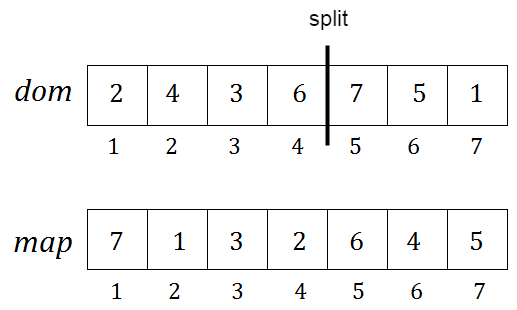
\includegraphics[scale=0.5]{images/sparseset.png}
\end{center}
\caption{A sparse set.}
\end{figure}
We cannot use this structure like that because the neighbourhood of a vertex doesn't form a suite of index. For example, if a vertex had three neighbours 8, 72 and 13, we can't directly know which vertex is contained in which index.
So we implemented a first data structure, the split array, which is a simplified version of the sparse set without \textit{map}. We also implemented an other structure, the sparse map, which is a sparse set with a hash map instead of an array for \textit{map}, permitting to associate a vertex with its position in \textit{dom}.
\newpage
\subsubsection{Split array}
A split array is composed only by the \textit{dom} array which contains all possible neighbouring vertices. The array is divided into two parts, one with the current neighbour vertices and the other one with the vertices which are not, or no more, neighbours. An integer value \textit{split} indicates the position of the array's separation.
\begin{figure}[H]
\includegraphics[width=7.5cm,height=4.5cm]{images/SplitArrayGraph.png}\hfill
\includegraphics[width=5cm,height=3cm]{images/SplitArray.png}
\caption{A graph with the split array of vertex 2.}
\end{figure}
To add a vertex (for example after sending units of flow on the path 0-1-2-4-5, an edge is created from 2 to 1 and 1 becomes a current neighbour of 2), we need to go through the right part of \textit{dom} to find the future neighbour vertex, exchange its place with the vertex on the right of \textit{split} and increase \textit{split} by 1. \newline

To remove a vertex, it is the reverse operation. We need to go through the left part of \textit{dom} to find the neighbour vertex, exchange its place with the vertex on the left of \textit{split} and decrease \textit{split} by 1.
\subsubsection{Sparse map}
A sparse map is a sparse set with a hash map instead of an array for \textit{map}. The hash map associate each vertex with its position in \textit{dom}.

To add or remove a vertex, it is the same as for the split array but we don't need to go through \textit{dom} because we can obtain the position of a vertex in \textit{dom} thanks to the hash map, saving valuable time. In compensation, we need to update the hash map so it remains consistent. We simply need to swap the values of the two vertices which were exchanged in \textit{dom}.
\newpage
\subsection{Complexities}

We use 5 functions on our data structures ;
\begin{description}
\item[entrySet] which is used to obtain the set of neighbours
\item[get/set] which, respectively, returns or modifies a capacity
\item[add/remove] which is used to add or to remove a vertex
\end{description}


This table below represents the complexities with the notation big O, which means "in the worst case". Although for the tree map, the simple linked list and the split array, the worst case is not too penalizing but that is not the case for the hash map and thus for the sparse map. Indeed, we obtain $O(n)$ if every elements of the hash map are in the same bucket. However, with a correct hash function, it should not arise. \newline
\begin{figure}[H]
\centering
\begin{tabular}{|c|c|c|c|c|c|}
	\hline
     & \textbf{Hash map} & \textbf{Tree map} & \textbf{Simple linked list} & \textbf{Split array} & \textbf{Sparse map}\\
     \hline	
   entrySet & $O(n)$ & $O(n)$ & $O(n$) & $O(n)$ & $O(n)$ \\
   get/set & $O(n)$ & $O(log$ $n)$ & $O(n)$ & $O(n)$ & $O(n)$ \\
   put & $O(n)$ & $O(log$ $n)$ & $O(1)$ & $O(n^-)$ & $O(n)$ \\
   remove & $O(n)$ & $O(log$ $n)$ & $O(n)$ & $O(n)$ & $O(n)$ \\
   \hline
\end{tabular} 
\end{figure}

With $n$ the number of outgoing edges of a vertex and $n^-$ the number of incoming edges. So, $n$ is also the number of neighbours.